\documentclass[12pt]{article} % font size can be 10, 11, or 12pt


%--------------------------------------------------------------------------------------------%
%       LOADS PACKAGES & CONFIGURES DOCUMENT STYLE        %
%--------------------------------------------------------------------------------------------%

\usepackage{amscd,amsmath,amssymb,amsthm} % --- used for typesetting mathematics 
\setlength\parindent{24pt}
\usepackage{caption}
\usepackage{subcaption}
\usepackage{cite}
\usepackage{graphicx}
\usepackage{listings}
\usepackage{float}
\usepackage{epsfig,psfrag,epstopdf} %--- useful if you include figures in your document
\usepackage{fancyhdr} %--- used for constructing headers and footers
\usepackage{lastpage} %--- used for reference to the last page number
\usepackage{graphicx,wrapfig} %--- used to include graphics
%\usepackage{wrapfig} %--- uncomment this line if want to allow in-line images
\usepackage{hyperref} %--- creates hyperlinks within the document with commands like \label{...}-\ref{...} and \cite{...} 
\usepackage{comment}
\usepackage{multirow}
\usepackage{xcolor}
\usepackage{amsmath}
\usepackage{wrapfig}    % inline figures
\usepackage{enumitem}
\usepackage{mwe} % Use for Images
\usepackage{here}     % Forced Figure Placement
\usepackage{pslatex}	% Use PostScript Fonts
\usepackage[utf8]{inputenc}
\usepackage{amssymb}
\usepackage{tabularx}


\hypersetup{pdfpagemode=FullScreen, linktoc=page, colorlinks=true, citecolor=blue, linkcolor=red, urlcolor=blue} %--- a basic setup for hyperref. 

% - declares math type environments
\newtheorem{theorem}{Theorem}[section]
\newtheorem{proposition}[theorem]{Proposition}
\newtheorem{lemma}[theorem]{Lemma}
\newtheorem{corollary}[theorem]{Corollary}
\newtheorem{question}[theorem]{Question}
\newtheorem{property}[theorem]{Property}

\theoremstyle{definition}
\newtheorem{claim}[theorem]{Claim}
\newtheorem{definition}[theorem]{Definition}
\newtheorem{conjecture}[theorem]{Conjecture}
\newtheorem{condition}[theorem]{Condition}
\newtheorem{remark}[theorem]{Remark}
\newenvironment{rem}{\begin{remark}\rm}{\end{remark}}
\newtheorem{example}[theorem]{Example}
\newenvironment{ex}{\begin{example}\rm}{\end{example}}
%%%%%%%%%%%%%%%%%%

\newcommand{\abs}[1]{\lvert#1\rvert}



% - changes the text boundaries on the page
\topmargin=-.5cm
\evensidemargin=0cm
\oddsidemargin=0cm
\textwidth=16.5cm
\textheight=21.5cm
\headsep=1cm
%%%%%%%%%%%%%%%%%%

% - configures header and footer
\linespread{1.2}
\newcommand{\heading}{\pagestyle{fancy}\lhead{Fu, Cui, Wei, Zhang} \rhead{Machine Learning in Severity Prediction}\cfoot{\thepage} 
\renewcommand\headrulewidth{0.4pt}
\renewcommand\footrulewidth{0.4pt}
\newcommand{\wkTitle}{Stress Testing} 
\newcommand{\AuthorName}{Anyi Fu, Xiwen Cui, Boyang Wei, Zhiming Zhang}}
\setlength\parindent{0pt}
%%%%%%%%%%%%%%%%%%%


%-----------------------%
% %%%%%%%%%
%-----------------------%
\begin{document}   %
%-----------------------%


%---------------------------%
%      TITLE PAGE      %
%---------------------------%

\title{
    \vspace{1cm}
        {\bf
        {\Large STATS 3ST3\\
        \vspace{2mm}Winter 2021\\[.3\baselineskip]
        \rule{\textwidth}{1.5pt}\vspace*{-\baselineskip}\vspace*{2pt}\\
        \rule{\textwidth}{0.4pt}\\[\baselineskip]
        \Huge \vspace{5mm}Machine Learning in Severity Prediction}\vspace{5mm}
        }\\
        \rule{\textwidth}{0.4pt}\vspace*{-\baselineskip}\vspace{3pt}
\rule{\textwidth}{1.5pt}\\[\baselineskip]
        \date{April 2021}\\
        \vspace{3cm}{
        \begin{center}
 \author{
Anyi Fu\\
400136866\\
\and
Boyang Wei\\
400104356\\
\and
Xiwen Cui\\
400144427\\
\and
Zhiming Zhang\\
400135152\\
}

\end{center}
        }
}

\maketitle
\thispagestyle{empty}
\pagestyle{empty} % - no header/footer on title page


%{\begingroup
%\centering % - centers everything on page
%{\Large \textsc{}}\\[.3\baselineskip]
%{\Large \textsc{Winter 2021}}\\
%\vspace*{2cm} % - vertical space 3cm
%\rule{\textwidth}{1.5pt}\vspace*{-\baselineskip}\vspace%*{2pt}
%\rule{\textwidth}{0.4pt}\\[\baselineskip]
%{\huge {\bf Machine Learning in Severity Prediction} \\ %[0.3\baselineskip] }\ % - your title goes here
%\rule{\textwidth}{0.4pt}\vspace*{-\baselineskip}\vspace{3pt}
%\rule{\textwidth}{1.5pt}\\[\baselineskip]
%\vspace*{6\baselineskip} % - vertical space between title and authors - 

%{\large Anyi Fu
%\\Xiwen Cui\\Boyang Wei\\Zhiming Zhang}
%\\[\baselineskip] 
        
% - NO STUDENT NUMBER!
%\vfill % - pushes the date and Abstract to the bottom of the page. If the abstract is long it will be pushed over the next page. To avoid this adjust the vertical space above the authors list. 
%{\today}\\[0.3\baselineskip] % - today's date. Change the \today to a set date if you want
%\abstract{abstract} % - abstract: replace \lipsum[1], keep the curly brackets {}
%\endgroup}

%-----------------------------------------%
%     TABLE OF CONTENTS      %
%-----------------------------------------%

\newpage % - new page
\thispagestyle{empty} %--- no heading on the Table of Contents page
\heading
\vskip3cm
\tableofcontents
\clearpage
\pagenumbering{arabic} %--- resets the page counter to 1 starting with the next page
\newpage

%--------------------------------%
%     BODY OF PAPER    %
%--------------------------------%

\section{Introduction}
Machine learning brings major changes to the way risks, claims, and customer experiences are handled by insurance companies. These companies are able to work with large amounts of data and identify important insights of the data thanks to machine learning\cite{sas_2021}. In this report, we will be adopting machine learning methods on two datasets provided by The Co-operators General Insurance Company to predict auto loss severity. 

\subsection{Background}
The Co-operators is a leading Canadian multi-line insurance and financial services co-operative with \$47.3 billion in assets under administration\cite{operators_2021}. Its companies provide services in four main areas: property and casualty (P&C) insurance, life insurance, institutional asset management and brokerage operations\cite{operators_2021}. The datasets that will be used in later parts of this report are taken from the final round of the Second McMaster \& Co-operators Problem Solving e-Workshop, organized by the Department of Mathematics \& Statistics at McMaster University and The Co-operators General Insurance Company. It consists 16995 profiles and 80 characteristics of the insureds. The main coverage used in these datasets are the auto Accident Benefits (AB) and the Third Party Liability (TPL).

\subsection{Supervised Learning and Classification}
Supervised learning, also know as supervised machine learning, is a subcategory of machine learning and artificial intelligence\cite{ibm_cloud_education_2020}. It is defined by its use of labeled datasets to train algorithms to classify data or predict outcomes\cite{ibm_cloud_education_2020}. There are two labeled dataset that is used in the process of supervised learning: a training set and a testing set. The training set, used to train a model, contains massive amount of inputs and its corresponding correct outputs. The testing set, used to test the trained model, contains input and output pairs that are independent to the training set. Ultimately, Our goal is to use this training set to teach our algorithms to yield an output with an acceptable correctness given a new input from the testing set\cite{brownlee_2020}.

\vspace{\baselineskip}
Classification is a supervised learning concept, used to draw conclusions on how an entity should be labelled\cite{ibm_cloud_education_2020}. In this report, we will predict loss severity by labeling whether a profile is a big loss or not. We will achieve this by using two most common classification methods: K-Nearest Neighbors and Random Forest.

\newpage
\section{Algorithms and Model Fitting}

\subsection{k-Nearest Neighbors}
The K-Nearest Neighbors (k-NN) algorithm is a simple implementation of supervised learning that can be used to solve both classification and regression problems. The k-NN algorithm takes on the moral that similar things are close to each other, as the famous saying says, "Birds of a feather flock together".

\begin{figure}[h]
    \centering
    \begin{subfigure}{.5\textwidth}
        \centering
        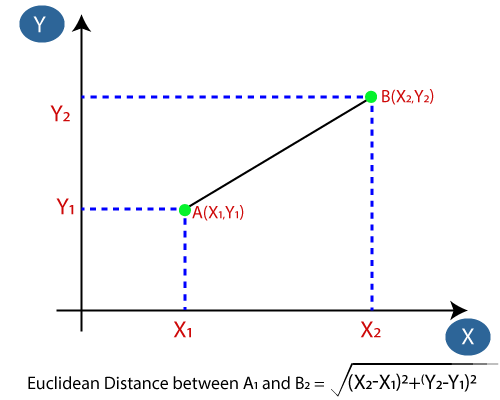
\includegraphics[width=\linewidth]{KNN/euclidean.png}
    \end{subfigure}
    \hfill
    \begin{subfigure}{.45\linewidth}
        \centering
        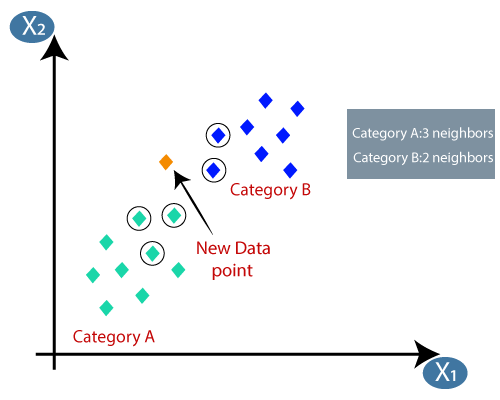
\includegraphics[width=\linewidth]{KNN/KNN.png}
    \end{subfigure}
    \caption{simple k-NN classification\cite{knn4}} 
\end{figure}

The most popular way to calculate the similarity or closeness between data points is by using Euclidean distance as shown above. Aside from being able to quantify the closeness, we also need some procedures to finally implement k-NN: \cite{knn3}

\renewcommand{\labelenumii}{\roman{enumii}}
\begin{enumerate}
    \item Initialize k number of nearest neighbors by running through each possible value for k and choose the optimal one with maximum accuracy or minimum error.
    \item For each input value:
        \begin{enumerate}
            \item Calculate the Euclidean distance between the current data and its query data point.
            \item Add the result and the index of the current data to an ordered list.
        \end{enumerate}
    \item Sort the ordered list consisting all distances and indices in ascending order by distances, and choose the first K data point from this sorted list.
    \item The input values will be assigned to the category that is most common among the k nearest neighbors.
\end{enumerate}

\subsubsection{Application in Python}
Owing to the fact that our dataset contains too many variables, we choose to drop variables that are relatively unimportant to predicting a loss severity and columns that contain too many null values. Among the remaining variables, some of them are categorical variables that take on the form of strings, as we can see in Figure 2.

\begin{figure}[h!]
    \centering
    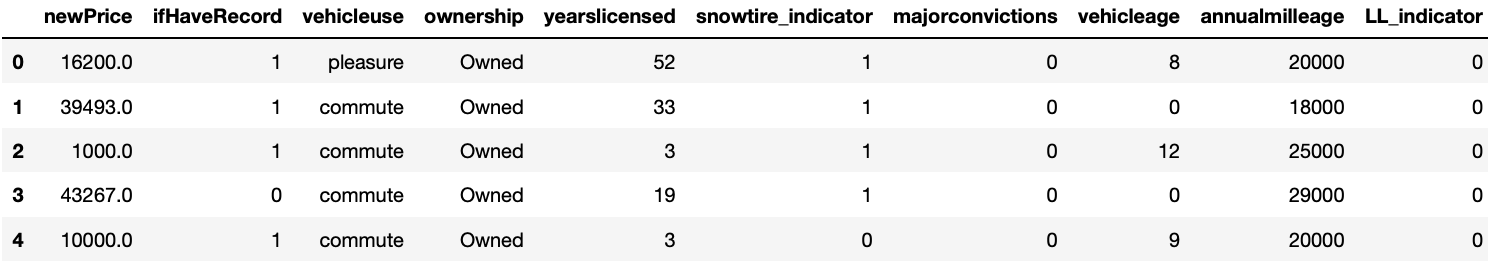
\includegraphics[width=0.9\linewidth]{KNN/trainSet.png}
    \caption{First five rows of training set}
\end{figure}

\begin{figure}[h!]
    \centering
    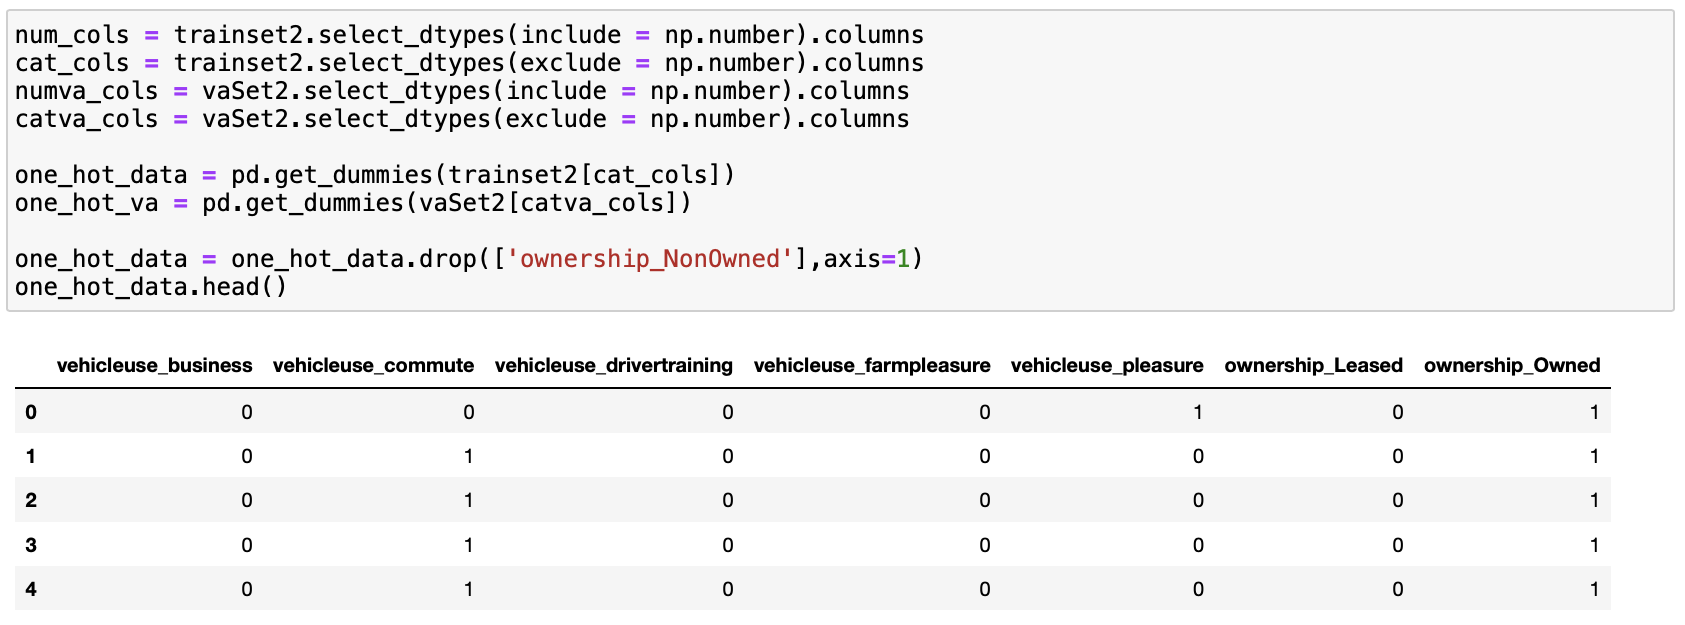
\includegraphics[width=0.9\linewidth]{KNN/onehot.png}
    \caption{New columns generated after one-hot encoding}
\end{figure}

In order to analyze these categorical variables mathematically, we first need to convert these categorical variable into numerical variable with binary values using one-hot encoding. As an illustration, because we know that the variable 'vehicleuse' takes on five categorical values: "pleasure", "business", "commute", "drivertraining", and "farmpleasure", we can create five new columns namely 'vehicleuse\_pleasure', 'vehicleuse\_business', 'vehicleuse\_commute', 'vehicleuse\_drivertraining', and 'vehicleuse\_farmpleasure' to hold an indicator of 1 or 0 representing a yes or no to that subcategory. For example, the initial vehicle use for the first insured at row 0 is pleasure, so as illustrated in Figure 3, the new corresponding value for 'vehicleuse\_pleasure' is 1, and all the other subcategories are 0.

\vspace{\baselineskip}
In addition to modifying the dataset, we decide to split 70\% of the dataset to use it as the train set and use the remaining 30\% as the test set. Particularly, we split this dataset into X\_train, X\_test, y\_train, y\_test using train\_test\_split() function. The reason for this decision is that we can use X\_train and y\_train to train the model and compare the predictions to y\_test to check the model's performance. we 

\vspace{\baselineskip}
After perfecting our datasets, we turn to implementing the k-NN algorithm. To make things easy, we simply import \emph{KNeighborsClassifier} from \emph{sklearn.neighbors package} instead of implement k-NN algorithm from scratch. To find parameter k, we write a function, shown in Figure 4, that computes each accuracy score for k from 1 to 20, and choose the one that is the most appropriate.


\begin{figure}[h!]
    \centering
    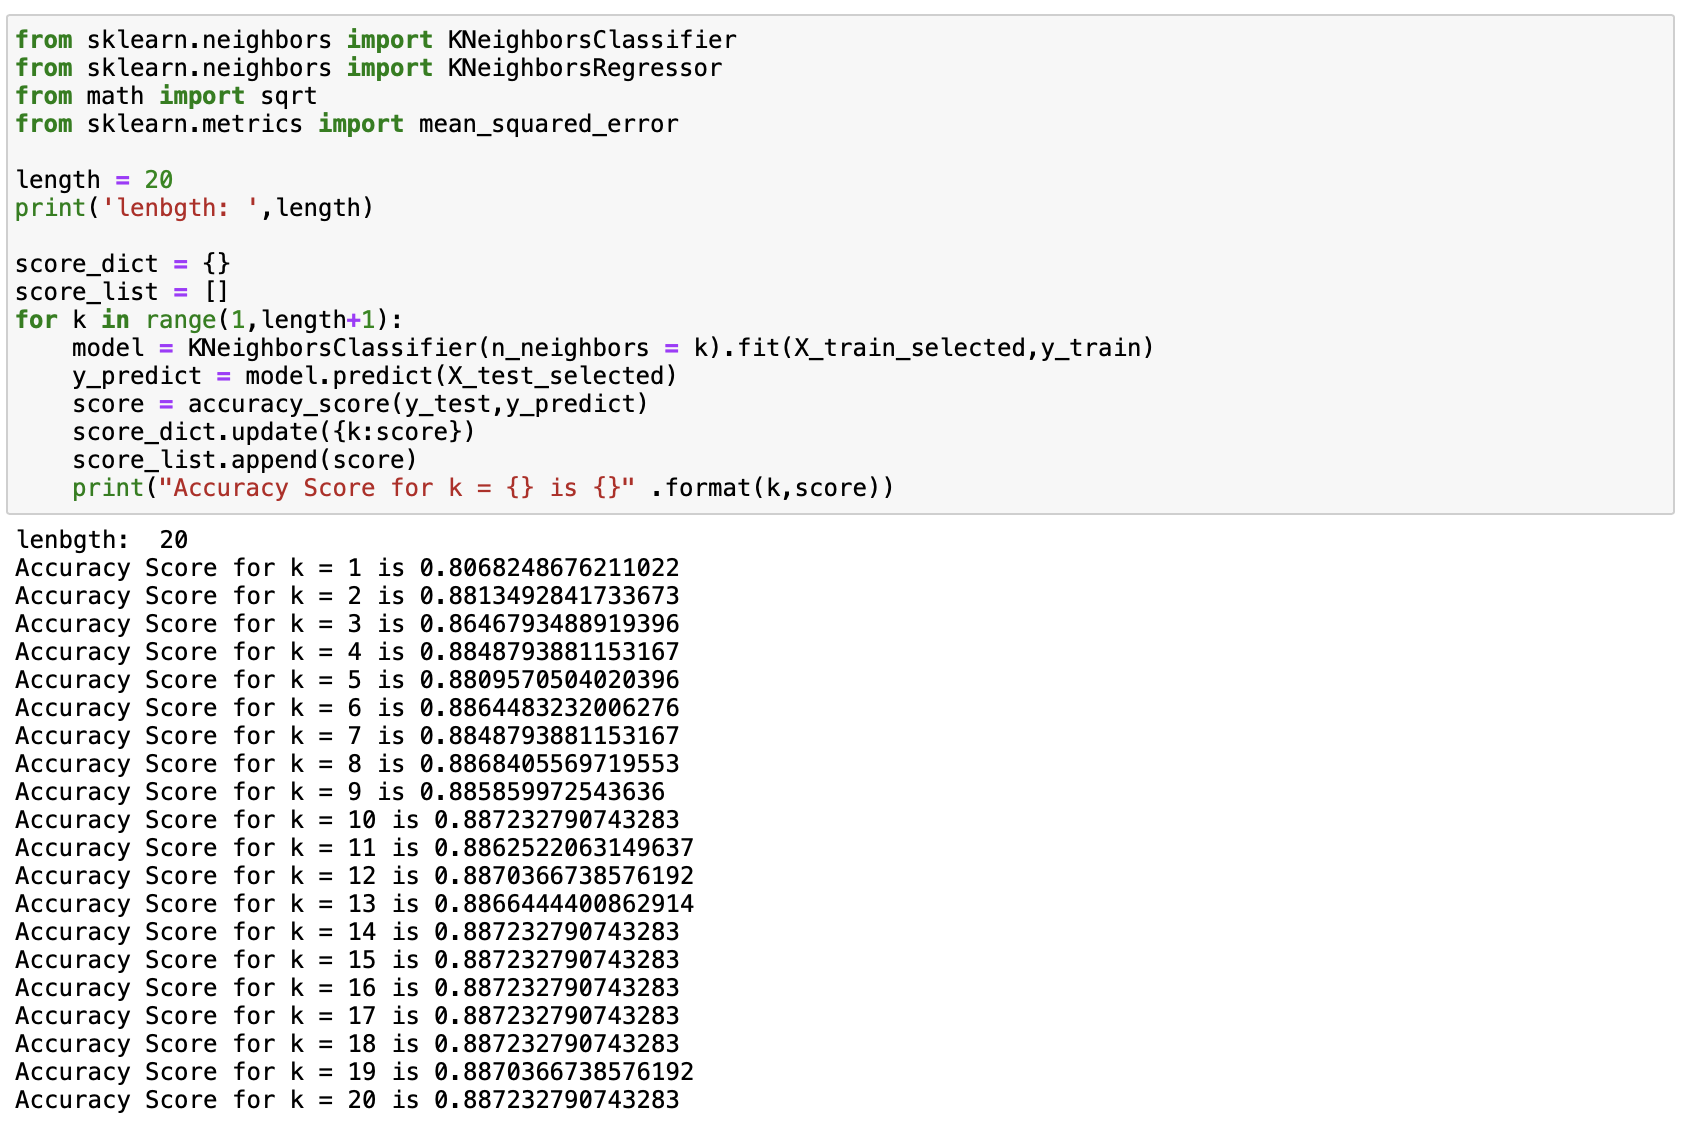
\includegraphics[width=0.8\linewidth]{KNN/k.png}
    \caption{Find parameter k through accuracy score}
\end{figure}


\subsubsection{Model Fitting and Validation}
Following the computation on all accuracy scores for k from 1 to 20, we plot these scores for a better analysis.

\begin{figure}[h]
    \centering
    \begin{subfigure}{.48\textwidth}
        \centering
        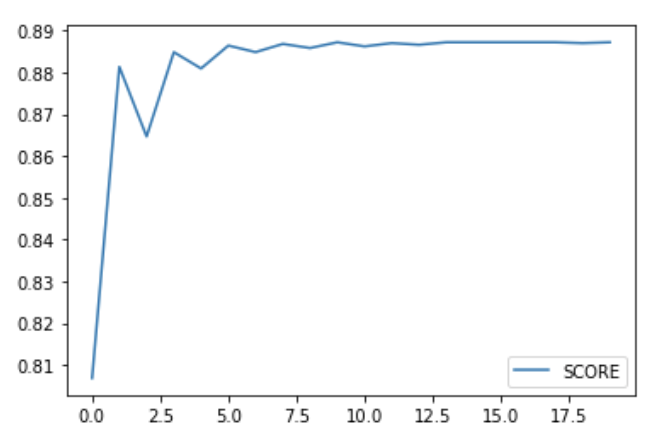
\includegraphics[width=\linewidth]{KNN/kplot.png}
        \caption{Accuracy scores for k from 1 to 20}
    \end{subfigure}
    \hfill
    \begin{subfigure}{.48\linewidth}
        \centering
        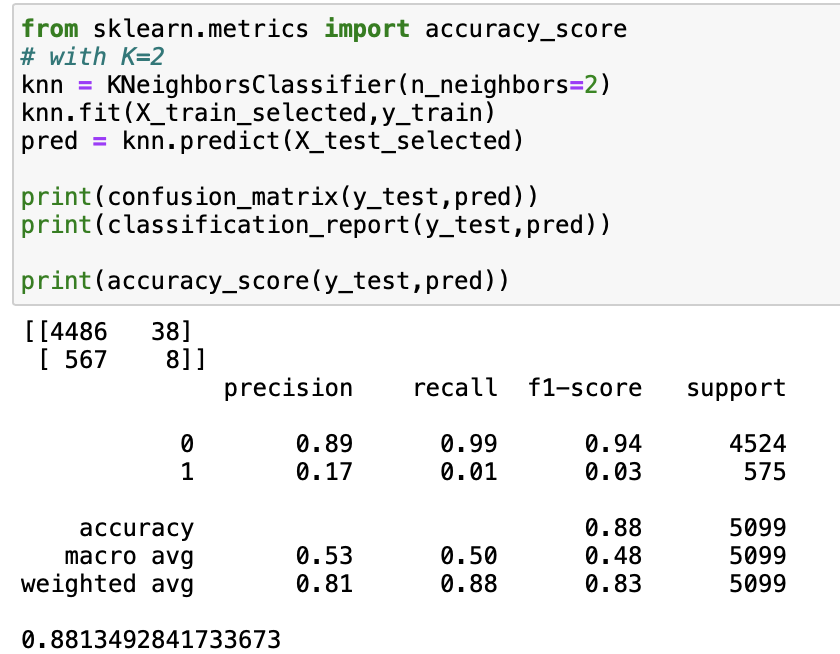
\includegraphics[width=\linewidth]{KNN/validate.png}
        \caption{Confusion matrix and classification report}
    \end{subfigure}
    \caption{}
\end{figure}

As illustrated in the Figure 5a above, the accuracy score dips at k = 3, then raises to about 0.885 at k = 4, and then succeeding to a constant trend. The classification boundaries seem to be smoother as k becomes larger, so to prevent over-fitting, k = 2 is being considered. From there on, the next step is to fit the model and compute confusion matrix and classification report. From the confusion matrix and classification report shown in Figure 5b, we see that 4486 out of 4524 values are predicted correctly in the class 0 (LL indicator for a small loss), however only 8 out of 575 values are predicted correctly in the class 1(LL indicator for a big loss). On the other hand, the overall f1-score is 0.88, which is not bad.

\vspace{\baselineskip}
Although the f1-score for class 0 is high, this score alone is not enough. For an insurance company, it is expected to precisely identify if an insured has potential high-severity. In this case, the accuracy in predicting class 1 insureds needs to be improved. One possible adaption is to add the dropped variables as they might contribute to the model fitting.

\newpage
\subsection{Random Forest}
Random forest is also a widely used supervised learning algorithm due to its simple and diverse nature. This algorithm can be used for both classification and regression tasks. Therefore, it can deal with qualitative, quantitative, or a mixed type of data set.

\subsubsection{Decision Tree}
To understand this algorithm better, we first go over how decision trees work using an example.\cite{RandomForest}

\begin{figure}[H]
    \centering
    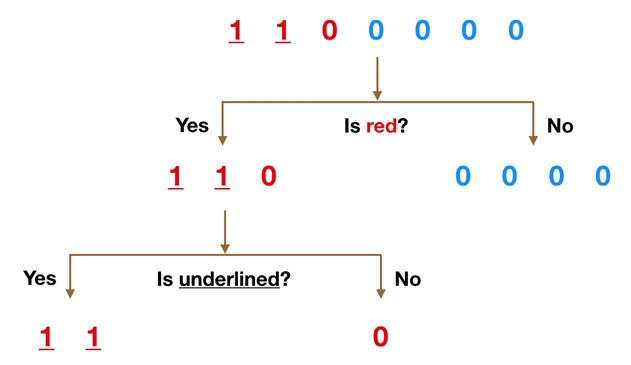
\includegraphics[width=8cm]{p1.png}
    \caption{Decision Tree}
    \label{fig:my_label}
\end{figure}

Imagine that our dataset contains those number at the top of the decision tree illustrated in Figure 6. Notably, there are some characteristics to these numbers. Now let’s say that our goal is to find out which observations exhibits the colour red and is also being underlined. We can start by checking if a given observation is red. This allows us to split all observations into two groups based on their color: red and blue. We can then check if a given observation is underlined. This allows us to further divide the two groups into two more groups each based on their underlying property: underlined and not underlined. As a result, we find that there are two observations in this decision tree that matches our goal. Ultimately, we are trying to capture all the patterns in a dataset, and this process is called the model fitting. Furthermore, we can feed new datasets to this fitted model and make predictions based on the same characteristics our training dataset exhibits. Obviously, our data won’t be as clean and simple as our exmample here in real life, but the logic to a decision tree remains the same. 

\begin{figure}[H]
    \centering
    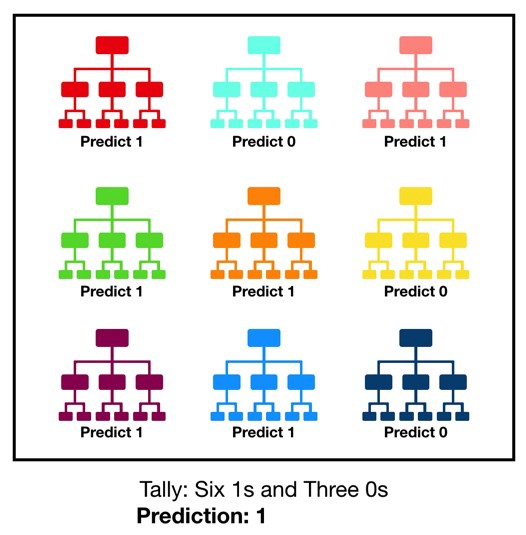
\includegraphics[width=8cm]{p2.png}
    \caption{Random Forest}
    \label{fig:my_label}
\end{figure}

\subsubsection{Random Forest}
A random forest is just a collection of decision trees. Each individual tree generate a class prediction and the class with the majority votes becomes our prediction model. In the case of Figure 7, Predict 1 is our prediction model because it has majority votes. Although the voting strategy can give us a more accurate and stable prediction, we still have to keep in mind that the correlation between each model has to be low, meaning our forest has to consist of only randomly created decision trees, to maintain precision.

\subsubsection{Application in R - Exploratory Data Analysis}
To start our analysis, we first load required packages into R, as shown in codes below. We then load our datasets into R. However, we notice that "Costnew" variable have null values that we'll need to take car of. Additionally, some of the variables we selected are categorical variables, so we decide to turn them into factor variables. This way, these variables can be implemented correctly in Random Forest modelling. Lastly, like the dataset used for k-NN, we split 70\% of the dataset as the train set and use the rest 30\% as the test set. Detailed coding on these modification is shown belown.

\begin{lstlisting}[language=R,xleftmargin=.1\textwidth]
library(magrittr)
library(tidyverse)
library(dplyr)
library(ggplot2)
library(randomForest)

trainset = read_csv('~/Desktop/workshop day package/
McMaster Workshop Train set.csv')
\end{lstlisting}

\begin{lstlisting}[language=R,xleftmargin=.1\textwidth]
# build a extract variables function
extractFeatures1 <- function(data) {
  features <- c("purchaseprice",
                "costnew",
                "vehicleuse",
                "ownership",
                "yearslicensed",
                "snowtire_indicator",
                "majorconvictions",
                "vehicleage",
                "annualmilleage")
  fea <- data[,features]
  fea$costnew[is.na(fea$costnew)] <- median(fea$costnew, na.rm=TRUE)
  fea$vehicleuse <- as.factor(fea$vehicleuse)
  fea$ownership <- as.factor(fea$ownership)
  fea$snowtire_indicator<-as.factor(fea$snowtire_indicator)
  fea$majorconvictions<-as.factor(fea$majorconvictions)
  return(fea)
}

index <- sample(nrow(trainset), 0.5*nrow(trainset), replace = FALSE)
trainset2 <- trainset[index,]
testset2 <- trainset[-index,]
\end{lstlisting}

\newpage
\subsubsection{Model Estimation and Evaluation}
Following the modification of datasets, we proceed to fit our model using Random forest algorithm. The code below gives us a summary of our result, shown in Figure 8. The out-of-bag error score gives us an unbiased prediction error of the model and we can see that our score is 11.09\%, which is not bad.

\begin{lstlisting}[language=R,xleftmargin=.1\textwidth]
rf <- randomForest(extractFeatures1(trainset2),
as.factor(trainset2$LL_indicator), 
ntree=500, mtyr=5,importance=TRUE)
\end{lstlisting}

\begin{figure}[H]
    \centering
    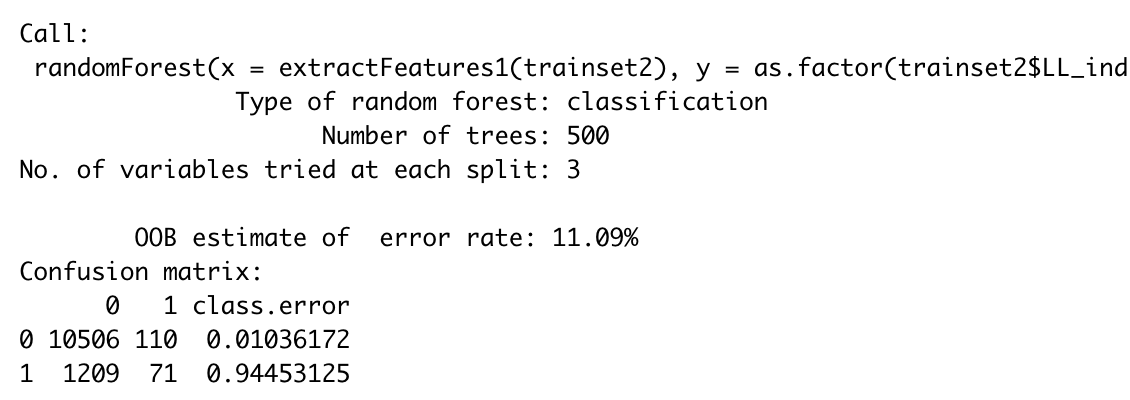
\includegraphics[width=8cm]{Type.png}
    \caption{Summary of random forest}
    \label{fig:my_label}
\end{figure}

We can also evaluate the importance of each variables by how much it decreases the mean accuracy and gini index. From our variable importance plot (Figure 9), we can see that the 3 most important variables are  "purchaseprice", "costnew", and "vehicleage". If we don't account one of these three variable, the mean accuracy and gini index will decrease at least 20\% each. Additionally, variables "yearlicensed", "ownership", and "vehicleuse" are also relatively important.

\begin{figure}[H]
    \centering
    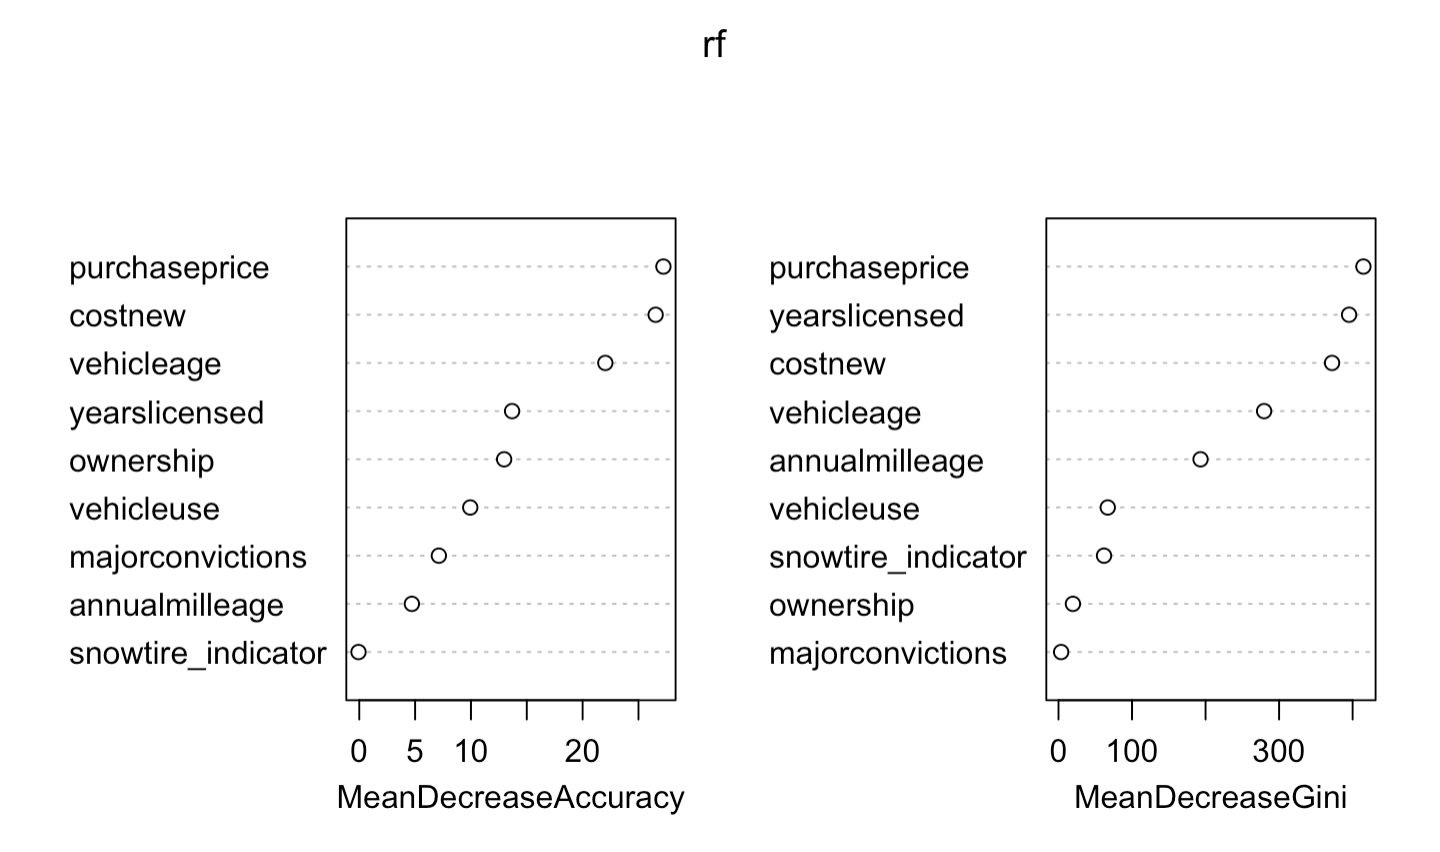
\includegraphics[width=8cm]{p4.png}
    \caption{Variance Importance Plot}
    \label{fig:subim2}
\end{figure}

\subsubsection{Validation}
Finally, we can predict the target variable(LL indicator) for our test dataset and evaluate the model's performance. Using the codes shown below, we get our confusion matrix graph\cite{confusionmatrix} shown in Figure 10. It is clear that only 60 class 0 predictions are wrong, and there are only 34 out of 538 class 1 predictions correct. Hence, the misclassification rate is bit high, but overall, the fitting performance is not bad since the error rate is below 12\%. 


\begin{lstlisting}[language=R,xleftmargin=.1\textwidth]
prediction<-predict(rf,newdata=extractFeatures1(testset2))
tab <- table(testset2$LL_indicator, prediction)
tab
1- sum(diag(tab))/sum(tab)
\end{lstlisting}

\begin{figure}[H]
    \centering
    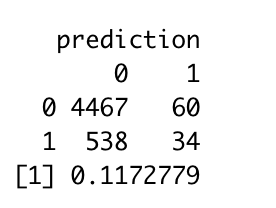
\includegraphics[width=8cm]{prediction.png}
    \caption{Confusion Matrix}
    \label{fig:my_label}
\end{figure}

In general, the performance is lower than what we expected. The misclassification rate is very high for predicting class 1 and it is not a good sign in an insurance company's point of view. Class 1 represents a high loss in a profile, so not able to predict them well is a bad thing. There are a lot of improvements that can be made in the future. One way to improve this model is by using cross validation method. This technique chooses the optimal parameters for our model instead of using the default values of the parameters in random forest function like what we did here. As a result, the error rate could be lower.

\newpage
\section{Conclusion}
\subsection{Summarization on k-Nearest Neighbors}
The k-Nearest Neighbor is a model that classifies data points based on their similarities. There are three key elements in k-NN:

\begin{itemize}
    \item The Euclidean distance calculation.
    \item The selection of k.
    \item The decision of classification.
\end{itemize}

Advantages of k-NN is applicable for both classification and regression. Firstly, k-NN is easy to implement, since it does not require training period to build a model. Secondly, the only required calculation in k-NN is the euclidean distances between different data points on the basis of different features.

\vspace{\baselineskip}
k-NN is called a lazy learner because it only memorizes the training dataset instead of learning a function from the training dataset. This means that no "training" is required in k-NN algorithm. Although this disadvantage can be seen as a convenience, it is not always beneficial for dealing with large datasets. Another disadvantage of k-NN is that the model is too sensitive to numbers of k\cite{KNN1}, which will affect prediction results. For example, a smaller k may lead to overfitting of the model. To explain further, because there are always some data points that belong to individual cases, the results may perform well on the training dataset but not on the new dataset. On the other hand, the classification boundary could be blurred and too smooth if k is too large. This is because if k is large enough to approach the number of data points in the dataset, the result becomes the frequency of occurrence of each data point and k-NN becomes meaningless. This is called underfitting and it causes model to perform poorly on the training data. Additionally, k-NN is not suitable for high dimensional datasets. Despite all of these disadvantages, k-NN algorithm is still used in various industries, such as forecasting stock market, credit rating in insurance, loan management in banking, and money laundering analyses\cite{KNN2}.

\subsection{Summarization on Random Forest}
Random forest is a typical algorithm of ensemble machine learning called bootstrap aggregation or bagging. There are three key elements in the following:

\begin{itemize}
    \item The weak generalization ability improves in decision tree.
\end{itemize}

\begin{itemize}
    \item The correlation between each tree is proportional to error rate.
\end{itemize}

\begin{itemize}
    \item The number of feature selection is proportional to correlation and classification ability.
\end{itemize}

One advantage of random forest algorithm is its diversity, it's applicable to both classification and regression problems. Another advantage is that random forest has the ability to deal with missing values in the dataset without affecting the accuracy of the fitting. The biggest advantage, however, is that random forest model does not over-fit as long as the data set is large enough, because it is a collection of decision trees and, therefore, it is insensitive to outliers.
Compared with k-NN, random forest can better handle large dataset with  higher dimensions. However, random forest algorithm also has some drawbacks. Random forest is effective for classification but not for regression. Furthermore, random forest algorithm suffers from the problem of interpretability of the decision trees, which is likely to lead to failure in determining the importance of each variable. As the number of decision trees in a random forest increases, the time required for training becomes larger, and since the algorithm builds numerous trees to combine their outputs, it also requires a lot of computational power.\cite{RF2}Despite its disadvantages, random forest can also be applied to various industries, such as fraud detection, stock movement, credit rating, product recommendations in e-commerce, and disease detection.\cite{RF1}


\subsection{Challenge to Machine Learning}
In modern society, machine learning algorithms have emerged in almost every industry, such as driverless cars, environmental forecasting, and financial management, all of which require algorithms to support their research. However, machine learning is based on big data, and model cannot be established without data. Therefore, while machine learning requires massive data to support its training process, the quality of data should also be good and unbiased. Meanwhile, in this process, a lot of personal privacy information and confidential documents will be exposed to the risk of leakage. For example, hackers can perform backward chaining on sensitive attributes of training data by interacting with the model. Therefore, the implementation of privacy protection in machine learning has become fundamental to the development of machine learning, and this issue has received increasing attention from the research community and industry.\newline

In conclusion, this report first introduces the methods of machine learning, including supervised learning and unsupervised learning. In addition, the advantages and disadvantages of machine learning are compared, and two different machine learning algorithms, k-NN and random forest, are implemented using the same dataset from the 2nd McMaster/Co-operators e-workshop, demonstrating their different algorithmic concepts and computational methods. From the result of the models, the errors suggest that the models may need new and stronger correlation variables to achieve better results. Today, as technology flourishes, challenges of machine learning also emerge, and data security and privacy protection will become important factors and development challenges in the future.

\addcontentsline{toc}{section}{References} %--- make the appropriate change here too 


\bibliographystyle{amsplain} 
%------------------ Adding the bibliography using dedicated software to create bib files: e.g., BibDesk on a Mac or equivalent for Windows...

\newpage
\bibliography{References.bib}
%--- the path /.../ to the bib file needs to be specified if the bib file is not in the same directory as the tex document



\end{document}